% THIS IS SIGPROC-SP.TEX - VERSION 3.1
% WORKS WITH V3.2SP OF ACM_PROC_ARTICLE-SP.CLS
% APRIL 2009
%
% It is an example file showing how to use the 'acm_proc_article-sp.cls' V3.2SP
% LaTeX2e document class file for Conference Proceedings submissions.
% ----------------------------------------------------------------------------------------------------------------
% This .tex file (and associated .cls V3.2SP) *DOES NOT* produce:
%       1) The Permission Statement
%       2) The Conference (location) Info information
%       3) The Copyright Line with ACM data
%       4) Page numbering
% ---------------------------------------------------------------------------------------------------------------
% It is an example which *does* use the .bib file (from which the .bbl file
% is produced).
% REMEMBER HOWEVER: After having produced the .bbl file,
% and prior to final submission,
% you need to 'insert'  your .bbl file into your source .tex file so as to provide
% ONE 'self-contained' source file.
%
% Questions regarding SIGS should be sent to
% Adrienne Griscti ---> griscti@acm.org
%
% Questions/suggestions regarding the guidelines, .tex and .cls files, etc. to
% Gerald Murray ---> murray@hq.acm.org
%
% For tracking purposes - this is V3.1SP - APRIL 2009

% require the `acm_proc_article-sp.cls` file.
\documentclass{acm_proc_article-sp}

\usepackage{url}
\usepackage{paralist}
\usepackage{graphicx}
\usepackage{subfigure}

\begin{document}

\newcommand{\framedots}{\framebox{\ldots}}

\title{Maintain-e-nator: \ttlit{Make the World a Better Place}}
%
% You need the command \numberofauthors to handle the 'placement
% and alignment' of the authors beneath the title.
%
% For aesthetic reasons, we recommend 'three authors at a time'
% i.e. three 'name/affiliation blocks' be placed beneath the title.
%
% NOTE: You are NOT restricted in how many 'rows' of
% "name/affiliations" may appear. We just ask that you restrict
% the number of 'columns' to three.
%
% Because of the available 'opening page real-estate'
% we ask you to refrain from putting more than six authors
% (two rows with three columns) beneath the article title.
% More than six makes the first-page appear very cluttered indeed.
%
% Use the \alignauthor commands to handle the names
% and affiliations for an 'aesthetic maximum' of six authors.
% Add names, affiliations, addresses for
% the seventh etc. author(s) as the argument for the
% \additionalauthors command.
% These 'additional authors' will be output/set for you
% without further effort on your part as the last section in
% the body of your article BEFORE References or any Appendices.

\numberofauthors{3} %  in this sample file, there are a *total*
% of EIGHT authors. SIX appear on the 'first-page' (for formatting
% reasons) and the remaining two appear in the \additionalauthors section.
%
\author{
% You can go ahead and credit any number of authors here,
% e.g. one 'row of three' or two rows (consisting of one row of three
% and a second row of one, two or three).
%
% The command \alignauthor (no curly braces needed) should
% precede each author name, affiliation/snail-mail address and
% e-mail address. Additionally, tag each line of
% affiliation/address with \affaddr, and tag the
% e-mail address with \email.
%
% 1st. author
\alignauthor
Xin Liu\\
       \affaddr{University at Buffalo}\\
       \affaddr{1932 Wallamaloo Lane}\\
       \email{xliu36@buffalo.edu}
% 2nd. author
\alignauthor
John Longanecker\\
       \affaddr{University at Buffalo}\\
       \affaddr{P.O. Box 1212}\\
       \email{john.longanecker@gmail.com}
% 3rd. author
\alignauthor
Juehui Zhang\\
       \affaddr{University at Buffalo}\\
       \affaddr{Hekla, Iceland}\\
       \email{larst@affiliation.org}
%\and  % use '\and' if you need 'another row' of author names
}

\maketitle

\begin{abstract}
Our system seeks to improve the quality of a facility as well as decrease an organization's overall operating expenses.  By letting those who maintain facilities know about problems sooner. Maintenance workers can react quicker and more efficiently if they have better information about the status of their facilities.  \textit{Maintain-e-nator} provides a cell phone application to report problems as well as a web interface to allow workers to manage and be notified of problems.
\end{abstract}

% A category with the (minimum) three required fields
\category{H.4}{Information Systems Applications}{Miscellaneous}
%A category including the fourth, optional field follows...
\category{D.2.8}{Software Engineering}{Metrics}[complexity measures, performance measures]

\terms{Applications}

%==========
% INTRODUCTION
%==========
\section{Introduction}
Eventually everything breaks. Nothing lasts forever. Buildings start as brand new but eventually break down.  Roads start as smooth, but eventually develop potholes.  These breakdowns can sometimes be ignored like a squeaky door, but others can cause safety and health risks. If the stairs of a building are in disrepair they could cause a tripping hazard for other people. The reasons for something not being fixed can vary. Budget, time, priority and awareness all play a role as to when thing get repaired. We seek to streamline the process at which maintainers become aware of problems.

%==========
% Motivation
%==========
\section{Motivations}
It is easy for a large organization to be unaware of all the maintenance problems that their facilities have. Some obscure room may need a light bulb replaced but those that work in that area do not report the problem or are not around when the problem is exhibiting its behaviors.  So the people who take a night class are the only ones aware of the problem.  They do not know where to submit a problem and are often not willing to do the necessary research to find out how to report a problem.

These problems are not limited to the inside of buildings. They can also involve roads, landscaping, sidewalks, and outdoor sports facilities. For example a pallet could fall off the back of a truck and be sitting in the middle of a road. Most drivers will drive around the pallet and not report it. People are not sure how to report a problem like this or it is not convenient to notify the people who maintain the road. Wouldn't it be nice if one could take out their cellphone and submit a report? Our version of \textit{Maintain-e-Nator} is targeted for the University at Buffalo's North Campus, but can easily be configured to be used in any setting.

\subsection{What is a problem?}
So far we have talked about what a problem is, but have yet to define what constitutes a problem. We consider a maintenance problem to be anything that can hurt someone as well as anything that detracts from the overall quality of a facility. At the end of the day the users who submits a problem are the ones who are deciding what a problem is.  Who better to determine a problem then those who actually use the facilities?  

\subsection{Goal}
The overall goal is to make maintenance workers aware of the problems that exists on their property. 
Are android application and web interface will not promise cleaner facilities. Our goal is to help those that manage a property.

%==========
% DESIGN
%==========
\section{Design}
Our application comprises of two parts: the Android application and the backend web application, which are designed for two kinds of users:
\texttt{submitters} and \texttt{maintainers}. Data flow can be depicted as Fig.~\ldots.

The data flow of our application is fairly intuitive: whenever a submitter spots some issues on a facility, they open up the Android application, which will
try to locate their position and generate a meaningful location ( such as a building name or the nearest mailing address), the submitters can take a few photos of the issue and record some audio regarding to the issue, then just hit the submit button, that's it! The rest for maintainers, they can use the web application to organize all the submitted issues, log their progresses on repair the issues. And if submitters choose to report the issues with their Google accounts, the backend can also update the issues status to submitters via email notifications automatically.

\subsection{Android Application}
We developed our client application on the Android~\cite{android} platform,
it is mainly consisted of three modules:
\begin{inparaenum}
 \item login module
 \item positioning module
 \item information collecting module.
 \end{inparaenum}
 Below we talk about these three modules in detail.
 \subsubsection{Login}
 Whenever some submitter wants to submit issues and open the application, she can choose to log in the application with her Google account or anonymously.
 We choose Google account because it is available in (or necessary for ) every Android device. We add some personal settings for users
 logs in with their Google accounts, and once the user submit some issue, the application will also pass her personal information (just name and email address)
 to our web application, which maybe used in the future for contacting with the user. With the \texttt{AccountManager} in Android library, we
 can only get the submitter's email address. To make our app more personalize, we want a little more of submitter's profile information.
 Once the submitter grant the application permission to retrieve her profile with the access token,
 we can use it to request the submitter information via calling UserInfo Google API~\cite{google-user-api}.
 This whole process follows the \texttt{OAuth2} specification~\cite{oauth2}.
 The application doesn't try to remember how the submitter logged in last time and use it for next time,
 each time submitter can choose whatever manner she wants.

\subsubsection{Positioning}~\label{sec:position}
 Each time when a submitter opens the application and files an issue, the application will start to request a single location update via 
 Network or GPS. We prefer Network update over GPS for it is much faster and accurate enough with the omni Wi-Fi APs within our campus.
 Also since it is unlikely for the submitter to move around when submitting an issue, we only request \textit{single} location update 
 to save battery life. \framedots
 
 Once the application gets the geolocation data, which is a pair of number for latitude and longitude, 
 we need to convert this geolocation into some meaningful information for the submitter.
 if the submitter is indoor (actually we will get the textual locations for both indoor and outdoor scenarios), 
 the application will try to guess which hall she maybe in by calculating the Euclidean distance between current geolocation 
 and the predefined geolocations of halls we current support, and assume the one with the nearest distance is the hall the submitter is in. 
 Otherwise, if the submitter is out of door, the application will try to get the meaningful location of the submitter by using 
 Google Place API~\cite{google-place-api} with the geolocation data, Currently we just use the first result returned by this API.
 
 Submitters can modify the location information suggested by the application later. Also, for outdoor scenario, 
 we implemented a \texttt{MapView} with a draggable marker which indicates submitter current position. 
 In some cases, if the geolocation provided is not that accurate or submitters move to another place after the location update, 
 they can adjust the position of marker, then the application will use that new geolocation accordingly.
 
 \subsubsection{Information collecting}
 For future maintainers to locate the issue position easily and accurately, we hope submitters can report the issue information
 as detail as possible. Since the location detail for indoor and outdoor could be very different, to ease the process of filling the detail
 of an issue, the application has two different forms for indoor and outdoor separately, as shown in Fig~\ref{fig:form}, 
 % TODO move to previous page
 \begin{figure*}[!t]
 \centering
 \subfigure{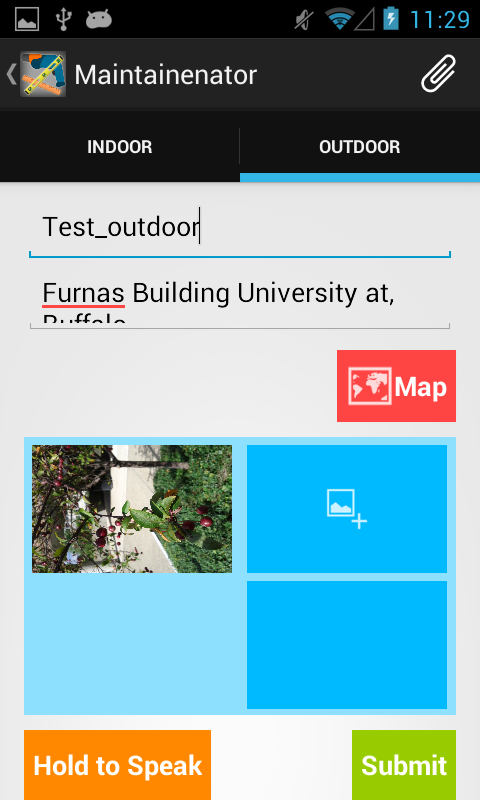
\includegraphics[scale=0.3]{images/outdoor_form.png}}
 \subfigure{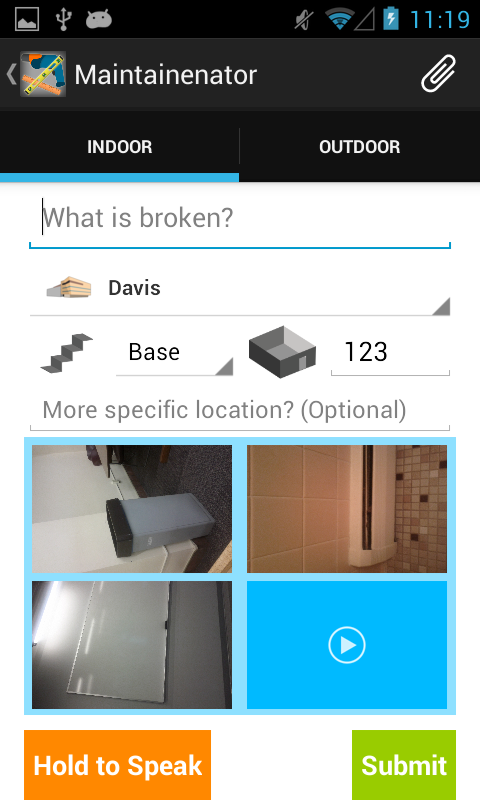
\includegraphics[scale=0.3]{images/indoor_form.png}}
 \caption{Issue form.} \label{fig:form}
 \end{figure*}
 The application requires submitter to at least provide a description, the location (which maybe acquired automatically as described in 
 Sec.~\ref{sec:position} or replaced by submitter). For current indoor experiment, we only support four halls - Davis Hall, Jarvis Hall, 
 Furnas Hall and Ketter Hall.

Only textual information may not be detail enough when describing an issue, thus we encourage submitter to add photos and 
also an audio recording regarding the location or issue detail. By long-pressing the image area,
the submitter can add up to three photos either from camera capture or gallery. After that the submitter can view the full-size photo by
clicking it and decide whether to keep it or replace it with a new one. For the audio recording, to make it act like a two-way radio,
we implement it as when submitter \texttt{holding} the recording button, the app will start record the audio until submitter release it.
We choose \texttt{wav} format for saving the audio recording because it is the quick and dirty way to enable the recorded
audio be played back both on the Android device and the browser.
The supported audio recording formats on Android (to our best knowledge), e.g., \texttt{mp4, 3gp} are not supported by current browsers. 
While the other formats supported by browsers without any plugins, e.g., \texttt{mp3, ogg} need third-party native libraries to be recorded on Android devices. 
For~\texttt{wav} format, after we collecting the raw audio data, we just need to wrap it up with~\texttt{wav} header, 
while the tradeoff is that file size is larger compared to those compressed formats.

\subsubsection{Others}
The application will save all the issues reported by the submitter locally on the Android device if the submitter choose to. Submitter can later
view the details of all the issues she reported before. We also add some animations to activity switching, users' interaction to make the application more accessible.

\subsection{Web Application}
For backend web service\footnote{\url{http://maintain-e-nator.herokuapp.com}}, 
we host our web application on \texttt{heroku}~\footnote{\url{https://www.heroku.com/}}, which is a
cloud application platform that saves us from all kinds of pitfalls in servers management, deployment. 
Since \texttt{heroku} does not store static files as well as users upload files, 
we use \texttt{Amazon S3}~\footnote{\url{https://aws.amazon.com/s3/}} for this task.

We use \texttt{Django}~\cite{django} web framework for our web application, its active community makes it easy and fast to develop web apps 
with numerous open source modules 
(a full list of all open source modules we used~\footnote{\url{https://github.com/forkloop/Maintainenator-backend/blob/master/requirements.txt}}). 
Our web application mainly has two components, private admin site, which is for maintainers to
manage all the reported issues, and public site, which is for every one to view existing reported issues.

\subsubsection{Private admin site}
\texttt{Django} is already packed with an admin module, which however is not that fancy,
We instead use \texttt{grappelli}~\footnote{\url{http://www.grappelliproject.com/}} for polishing up the admin
interface. The admin site is the main entry for maintainers, which allows multiple maintainers to manage the reported issues, 
filter them based on the issues location, severity level, status, submitted date \textit{etc}.
With the embedded Google Maps, maintainers can get an better idea of where the issues are for outdoor problems.
Also, the submitted photos and audio recording can give them more direct intuitions of what the issues are.
Maintainers can also keep tracking of their working progress for issues by add logs. Once there is an update for an issue, the web application
will send an email notification to the submitter if there is one. Currently, we only send notification to submitter once the issue is fixed.
 
\subsubsection{Public site}
The web application also has a public site that is intended for all to browse existing issues.
Inspired by \texttt{Pinterest, Airbnb} and other similar websites, we work on this public site to make it as an Single-page application~\cite{wiki-spa}, 
which can offer users a better experience with the infinite-scrolling, no more page reloading when viewing different issues. 
This is done by adding a model-view-controller (MVC) layer to user browser, and we use \texttt{Backbone.js}~\footnote{\url{http://backbonejs.org/}} 
as our frontend MVC. When user first open this public site, it starts to render a page and fetch the required data asynchronously from web application RESTful
API, with user scrolling down for more, it continues pre-fetching more data. Its ability to redraw any part of the UI without requiring a server roundtrip to retrieve
HTML makes it more-native-app-like~\cite{spa-book}.
The whole interaction with the backend is via the web application RESTful JSON interface. 

\subsubsection{Others}
The web application provides a RESTful API, which the Android application uses to submit an issue, or the public site uses to retrieve the issues
information. We use \texttt{tastypie}~\footnote{\url{http://tastypieapi.org/}} to build this REST-style interface. We did little hack on \texttt{tastypie}
for this API to support file upload via \texttt{mixin}.

Because \texttt{heroku} doesn't store user uploaded files, we use \texttt{Amazon S3} to store the photos and audio recording uploaded by submitters.
With \texttt{boot}\footnote{\url{http://docs.pythonboto.org/}}, we can achieve the transfer of uploaded files from \texttt{Heroku} to \texttt{Amazon S3}
transparently, once the web application receives a file from submitter, it is written to \texttt{Amazon S3} directly.

Normally, for a web application, besides handling income requests, it has other tasks like preprocessing uploaded images, sending emails to registered users,
and you don't want to mix these kinds of slow processes with HTTP handlers, for this would greatly slow down the request-response cycle, jeopardize users
experience. Thus we separate these kinds of tasks to other processes,
and use \texttt{foreman}\footnote{\url{http://ddollar.github.com/foreman/}} to manage them all.
There are two kinds of processes for our web application, the \texttt{web process} is for responding all HTTP requests, either rendering a view or
return some JSON data. While the \texttt{worker process} is for all other not emergent tasks, \textit{e.g.}, sending submitters emails regarding the issues they
submitted.

%==========
% TEST
%==========
\section{Test}
We developed and tested our Android application on Google Nexus S with 4.1.2 version. The Android application should also work fine on the
4.0.* platform. The location suggested \framedots
The source codes for both Android application\footnote{\url{https://github.com/forkloop/Maintain-e-nator}} and
web application\footnote{\url{https://github.com/forkloop/Maintainenator-backend}} are available on \texttt{github}.
%==========
% FUTURE WORK
%==========
\section{Future Work}
Though our application \ldots, there are a lot room for future improvement.
\begin{inparaenum}
 \item Current we didn't compress the photos and audio recording when sending them to the web application, which maybe consume a lot of data if the
 phone doesn't connect to Wi-Fi. To fix this, we can resize down the photos, and use a compressed audio format for recording the audio. Or we can allow
 submitters save current report and submit it later when they have Wi-Fi connection.
 \item The web application admin site is still \ldots, some functions like collapse the same issues reported by different submitters, allow issues fixing
 assignment to maintainers.
 \item We only tested the application within three of us, in the future, we can utilize \texttt{PhoneLab}~\footnote{\url{http://www.phone-lab.org/}} to
 fully test our application.
\end{inparaenum}

%==========
% CONCLUSION
%==========
\section{Conclusions}
Maintenance issues have been an annoying problem for many years. People may find some issues nearby but they don't know how to report them. 
We propose a new android application called \texttt{Maintain-e-Nator}, to make it easy for people to report their issues. People can choose indoor or outdoor, 
write down the description of problem, take at most three pictures, and even do some recording. We also build a web application, 
which is used by maintainers to manage the reported issues, filtering them based on the location, severity level, status, submitted date etc. 
Maintainers can view the issues locations on Google Maps, get an idea of what the issues are via submitted photos and audio recording.

%==========
% ACKNOWLEDGE
%==========
\section{Acknowledgments}
We would like to thank Prof. Steven Y. Ko and Prof. Geoffrey Challen for their valuable suggestions. We would also like to thank 
PhoneLab for providing us Android phones.

\bibliographystyle{abbrv}
\bibliography{sigproc}
\balancecolumns

\clearpage
\appendix
\section{Accomplishments}
Here we list our accomplishments for each milestone, 
the slides for each milestone demo can been viewed in \texttt{speakerdeck}\footnote{\url{https://speakerdeck.com/forkloop/cse622-milestone-reports}}.
\subsection{Milestone 1}
\begin{itemize}
\item
Set up the web application on \texttt{heroku}, has a simple public site.
\item
Develop the first version of Android application which is able to send some textual information and one photo to backend web application.
\end{itemize}

\subsection{Milestone 2}
\begin{itemize}
\item
Rewrite \texttt{FormActivity} with \texttt{Fragment}, separate indoor and outdoor information form.
\item
Tweak on Android application, handle special scenarios when there is no location update, or network connection.
\item
Separate photo from issue model, allows multiple photos upload.
\item
Allow submitter to save submitted issues.
\item
Add admin site to web application.
\end{itemize}
\subsection{Milestone 3}
\begin{itemize}
\item
Fully UI polishing for Android application, with designed icons, image buttons, new login activity, etc.
\item
Add audio recording function, allow submitter to also submit a short audio.
\item
Add a \texttt{MapView} to outdoor for submitter to adjust their location with Google Map interactively.
\item
Rewrite public site as Single-page application.
\end{itemize}
% That's all folks!
\end{document}
